This chapter describes the multicore aspects of LM's virtual machine and
provides a detailed experimental evaluation. First, we describe how local node
computation and parallelism are integrated, with a focus on locking and memory
allocation, and then we evaluate the performance, memory usage and scalability
of our implementation.

\section{Parallelism}\label{sec:implementation:parallelism}
A key goal of our parallel design is to keep the threads as busy as possible and
to reduce inter-thread communication. Initially, the VM partitions the
application graph of $N$ nodes into $T$ subgraphs (the number of threads) and
then each thread will work on their own subgraph.  During execution, threads can
steal nodes of other threads to keep themselves busy. The load balancing aspect
of the system is performed by our work scheduler that is based on a simple work
stealing algorithm. The pseudo-code for the main thread loop is shown in
Fig.~\ref{alg:thread_work_loop}. In each round, a thread inspects its work queue
for \emph{active nodes}, which are nodes with new candidate rules and, if there
is any, procedure \texttt{process\_node()} performs computation at the node
level. If the work queue is empty, the thread attempts to steal half of the
nodes from another thread. Starting from a random thread, it cycles through all
the threads to find one active thread. Eventually, there will be no more work to
do and the threads will go idle. There is a global atomic counter, a global
boolean flag and one state flag for each thread that are used to detect
termination. Once a thread goes idle, it decrements the global counter and
changes its flag to idle. If the counter reaches zero, the global flag is set to
idle. Since every thread will be busy-waiting and checking the global flag, they
will detect the change and stop executing.

\begin{figure}
\begin{algorithm}[H]
   \KwData{Thread TH, THREADS}
   \While{true}{
      $node \longleftarrow TH.work\_queue.pop\_node()$ \;
      \uIf{$node$}{
         $TH.process\_node(node)$\;
      }
      \Else{
         \tcc{Need to steal some nodes.}
         $target \longleftarrow random(len(THREADS))$\;
         $i \longleftarrow 0$\;
         \For{$i < len(THREADS)$}{
            $target \longleftarrow (target + 1) \% len(THREADS)$\;
            $nodes = THREADS[target].steal\_half()$\;
            \If{$len(nodes) > 0$}{
               $TH.work\_queue.add\_to\_queue(nodes)$\;
               break\;
            }
            $i \longleftarrow i + 1$\;
         }
         \If{$len(TH.work\_queue) == 0$}{
            \tcc{try to terminate}
            $TH.become\_idle()$\;
            \If{$TH.synchronize\_termination()$}{
               \Return{}\;
            }
            \tcc{There's new nodes in the queue.}
            $TH.become\_active()$\;
         }
      }
 }
\end{algorithm}
\caption{Thread work loop: threads process active nodes from the work queue
   until no more active nodes are available. Node stealing using a \emph{steal
      half} strategy is employed when the thread has no more active nodes.}
 \label{alg:thread_work_loop}
\end{figure}

Figure~\ref{fig:implementation:vm_overview} presents the layout of our virtual
machine for a program with six nodes and two running threads. Each thread space
includes the nodes owned by the thread (the dotted arrows represent the edges
between nodes) and a \emph{Work Queue}, which contains \emph{active nodes},
i.e., nodes that have new facts to process, and can be implemented as a simple
linked list. Initially, the \emph{Work Queue} is filled with all the nodes of
the thread in order to derive the initial facts.
Figure~\ref{fig:implementation:vm_overview} also illustrates the internal
structure layout of a node, which includes: the database of linear facts
(\emph{Linear DB}); the database of persistent facts (\emph{Persistent DB}); the
rule matching structures (\emph{Rule Engine}); and an auxiliary buffer for
storing intermediate facts coming from other threads (\emph{Fact Buffer}).

\begin{figure*}[t]
\centering
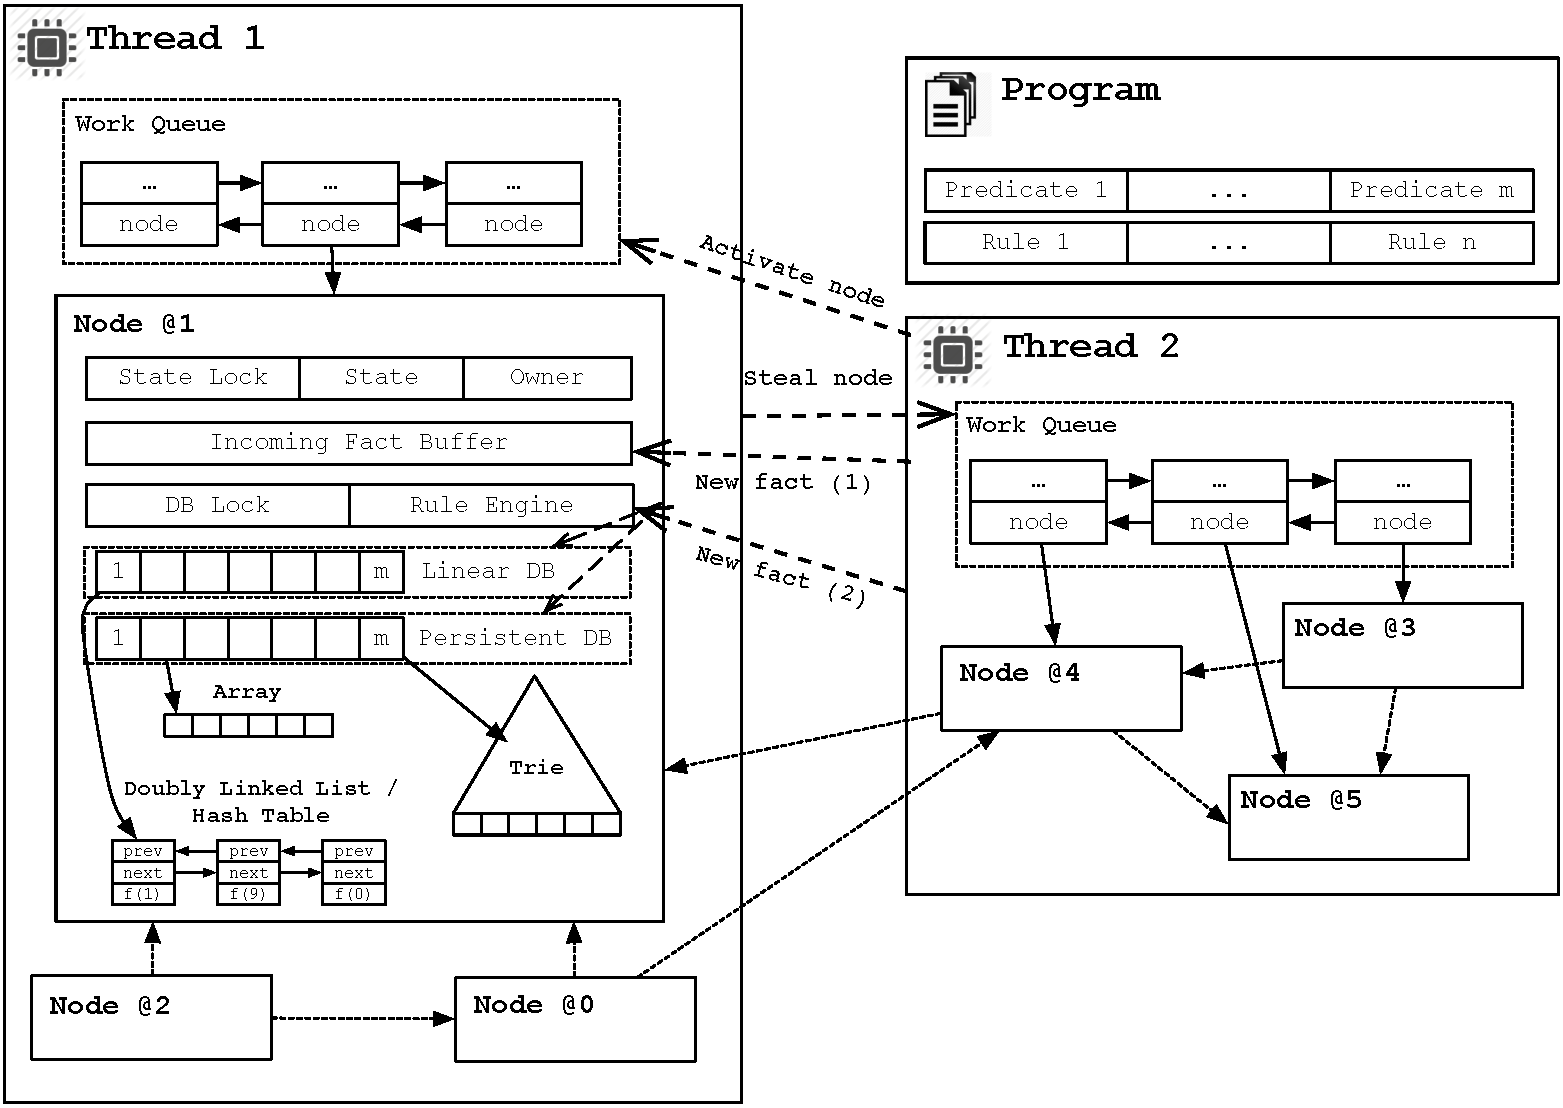
\includegraphics[width=\textwidth]{figures/implementation/vm_overview.pdf}
\caption{Layout of the virtual machine. Each thread has a work queue that
   contains active nodes (nodes with facts to process) that are processed one
   by one by the thread. Communication between threads happens when nodes
   send facts to nodes located in other threads.}
\label{fig:implementation:vm_overview}
\end{figure*}

Whenever a new fact is derived through rule derivation, we need to update the
data structures for the corresponding node. This is trivial if the thread that
derived the fact also owns the node. If that is not the case, then we have to
synchronize since multiple threads might be updating the same node's data
structures. We added a lock and a boolean flag to each node to protect the
access to its data structures. When the flag is activated, it means that the
node is currently being executed by the owning thread. For example, in
Fig.~\ref{fig:implementation:vm_overview}, if thread 2 derives a fact to node
\texttt{@1} (owned by thread 1), then thread 2 checks the node's flag and if not
activated, will lock node \texttt{@1} and perform the required updates
(\emph{New fact (1)}). If the flag is activated, it will not touch the main node
data structures, but instead will add the new fact to \emph{Fact Buffer}
(\emph{New fact (2)}). The facts stored in \emph{Fact Buffer} will then be
processed whenever the corresponding node's flag becomes active.

There is another thread interaction that might happen during fact derivation if
the node receiving a new fact is not active. In such case, the sending thread
needs to activate the node by pushing it to the \emph{Work Queue} of the target
thread. For example, consider again the situation in which thread 2 sends a new
fact to node \texttt{@1}. If node \texttt{@1} is not active, then thread 2 also
needs to activate \code{@1} by pushing it to the \emph{Work Queue} of thread 1.
After this synchronization point, the target thread is ensured to be active and
with a new node to process.

\subsection{Runtime Data Structures And Garbage Collection}

LM supports recursive types such as lists, arrays and structures. These compound
data structures are immutable and shared between multiple facts. Such structures
are stored in the heap of the VM and are managed through reference counting. For
instance, each list is a \emph{cons cell} with 3 fields: \texttt{tail}, the
pointer to the next element of the list; \texttt{head}, the element stored by
this element of the list; and \texttt{refs}, which counts the number of pointers
to this list element in the VM. The list is deleted from the heap whenever
\texttt{refs} is decremented to zero.

Nodes are also subject to garbage collection. If the database of a node becomes
empty and there are no references to the node from other logical facts, then the
node is deleted from the program. We keep around a small number of freed nodes
that can be reused immediately if another node is created.  We avoid garbage
collection schemes based on tracing since objects are created and discarded in
very specific points of the virtual machine and the runtime objects cannot
contain circular references. A reference counting mechanism is thus more
appropriate than a parallel tracing garbage collector which would entail pausing
the execution of the program to garbage collect all the unused objects.

In order to protect these important synchronization points, we use ticket
spin-locks. In Section~\ref{sec:data_structures} describes the locks used to
protect the node data structures. In addition to these locks, we also have a
lock per queue data structure that protects the thread's work queue.

In order to manipulate the state flag of each thread (see
Section~\ref{sec:implementation:parallelism}) we do not use locks but instead
manipulate the state flag using lock-free \emph{compare-and-swap} operations to
implement a state machine.

Finally, we summarize the synchronization hotspots by describing how the locks
are used in order to implement those hotspots.

\begin{description}

   \item \textbf{New Facts}: We use the node's \emph{Main Lock} and then attempt
      to lock the \emph{DB Lock}. If the \emph{Db Lock} cannot be used, then the
      new facts are added to the \emph{Fact Buffer}, otherwise the node data
      structure is updated with new facts. If the target node is not currently
      in any work queue, we lock the destination work queue and then add the
      node and change the state of the node to \textbf{active}. Finally, if the
      target thread that owns the target node is \textbf{idle}, we activate it
      by updating its state flag.

\item \textbf{Node Stealing}: For node stealing, we acquire the lock of the
   target thread's queue and then copy the stolen node pointers to a temporary
   buffer. For each node, we use the \emph{Main Lock} to update its
   \emph{Owner} attribute and then add it to the thread's work queue.

\end{description}


\section{Runtime Data Structures And Garbage Collection}

LM supports recursive types such as lists, arrays and structures. These compound
data structures are immutable and shared between multiple facts. Such structures
are stored in the heap of the VM and are managed through reference counting. For
instance, each list is a \emph{cons cell} with 3 fields: \texttt{tail}, the
pointer to the next element of the list; \texttt{head}, the element stored by
this element of the list; and \texttt{refs}, which counts the number of pointers
to this list element in the VM. The list is deleted from the heap whenever
\texttt{refs} is decremented to zero.

Nodes are also subject to garbage collection. If the database of a node becomes
empty and there are no references to the node from other logical facts, then the
node is deleted from the program. We keep around a small number of freed nodes
that can be reused immediately if another node is created. We avoid garbage
collection schemes based on tracing since objects are created and discarded in
specific points of the virtual machine. A reference counting mechanism is thus
more appropriate than a parallel tracing garbage collector which would entail
pausing the execution of the program to garbage collect all the unused objects.

\section{Memory Allocation}\label{section:implementation:allocation}

Memory allocation in the VM is extremely important because there is a need to
repeatedly allocate and deallocate logical facts. Logical facts tend to be small
memory objects, requiring, on average, 24 to 30 bytes of memory, which may lead
to fragmentation if allocation is not careful.  Moreover, since VM is
multithreaded, allocation also needs to be scalable, therefore using the
standard \code{malloc} facility provided by the POSIX standard may not be the
best idea since each operating system uses a different implementation that may
or may scale well in multithreaded environments.

\begin{figure}[ht]
   \begin{center}
      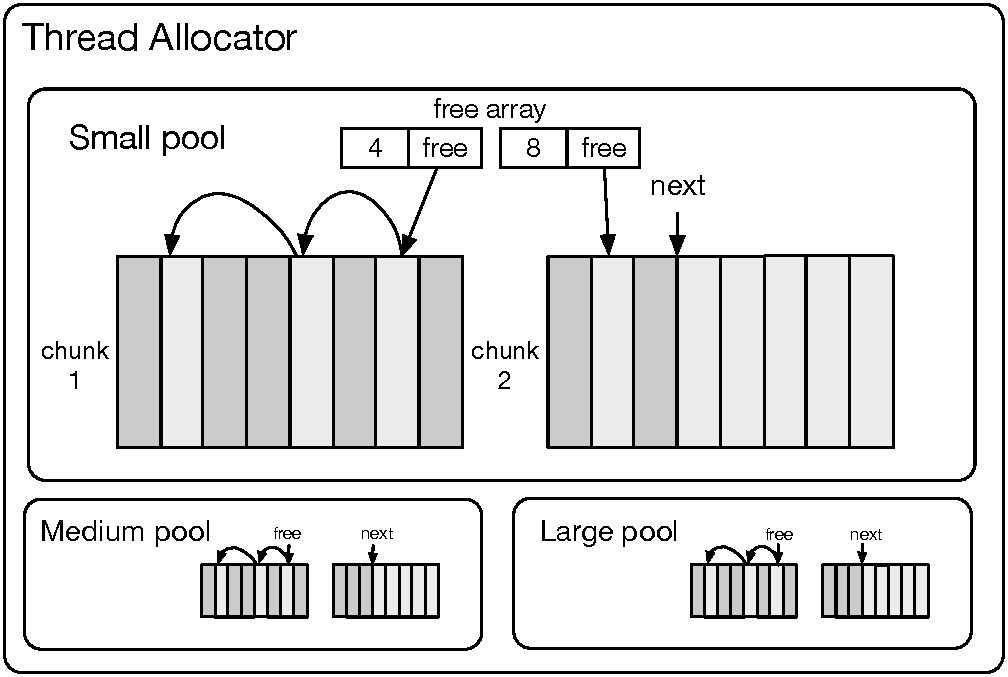
\includegraphics[width=0.7\linewidth]{figures/implementation/pool.pdf}
   \end{center}
   \caption{Thread allocator: each thread has a pool of slabs for allocating
      data structures. Each object size has: (1) several slabs that store contiguous chunks of
      memory of the same size; (2) a free list \code{free} of chunks that were freed; and (3) a \code{next} pointer that points to the next available free chunk.}
   \label{fig:implementation:pool}
\end{figure}

In order to solve these two issues, we decided to implement an allocator based
on the SLAB allocator~\cite{Bonwick-94}. SLAB allocation is a memory management
technique created in the Solaris 5.4 kernel used for efficiently allocate kernel
objects. Its advantages include reduced fragmentation and improved reuse of
deallocated data structures since these are reused in newer allocations.

Our particular implementation is presented in Fig.~\ref{fig:implementation:pool}
We pre-allocate multiple pools of memory chunks. We create one pool per object
size or data structure and each pool allocates large contiguous chunks of memory
that contain multiple objects of the same size. When allocating a particular
data structure, we first lookup the pool that
handles objects of the fact size and then check if there is an available object
in the chunks of memory. If all the chunks are empty, we use the \code{next}
pointer to allocate a new object inside a chunk. If there is no available space
in the chunk pointed by \code{next}, then we allocate a bigger chunk. We also
have a pointer \code{free} that points to deallocate objects and which creates a
list of free objects inside the available chunks. If the list has free objects,
we use the object pointed by \code{free} and update the \code{free} pointer
accodingly.

In order to reduce thread contention in the allocator, each thread uses a
different instance of the threaded allocator. When a thread wants to allocate an
object, it asks its own allocator for a new object. When deallocating, a thread
may deallocate an object that is part of another thread's allocator. However,
this is not an issue since chunks are not garbage collected from the system,
which allows another thread to reuse the pointer for a later allocation.

\iffalse
\subsection{Fact Allocation}

Although threads only allocate from their own memory chunks, they may reuse
objects from chunks created by another thread. Consider the following sequence
of events: (1) thread \code{T1} allocates multiple facts for node \code{A} in
the memory chunk \code{C1}; (2) thread \code{T2} executes node \code{A} and
allocates several facts in its own memory chunk \code{C2}; (3) thread \code{T1}
executes \code{A} again and needs to iterate through \code{A}'s facts which are
located in different multiple chunks, resulting in poor memory locality and
increased cache line misses. It is obvious that, in a perfect scenario,
\code{A}'s facts should be placed in a contiguous memory area in order to reduce
cache misses.

To tackle these issues, we have implemented a per-node fact allocator that is
implemented on top of the threaded allocator. The fact allocator allocates
chunks of memory from the main allocator which are then used to allocate facts
for that particular node. When a thread needs to allocate or deallocate a fact,
it acquires the allocator lock of the target node's allocator and performs the
allocation operation. Each fact allocator can allocate multiple chunks of
memory, depending on the amount of required facts. There is a doubly-linked list
of memory chunks and each chunk contains facts of different sizes (predicates).

Figure~\ref{fig:implementation:fact_allocator} presents an example state of a
fact allocator. The node has 3 memory chunks, all connected using the
\code{next} and \code{prev} pointers. Each chunk also has a reference count
(\code{refcount}) of the facts allocated in the chunk. If the reference count
ever drops to zero, then the memory chunk is deallocated. Deallocated facts are
kept on an array of linked lists named \code{free\_list} (contiguous in the
chunk, not as separate data structure), where each position of the array is a
linked list for facts with the same size. When allocating a new fact, we use the
first element of the linked list for facts with the same size.

\begin{figure}[ht]
   \begin{center}
      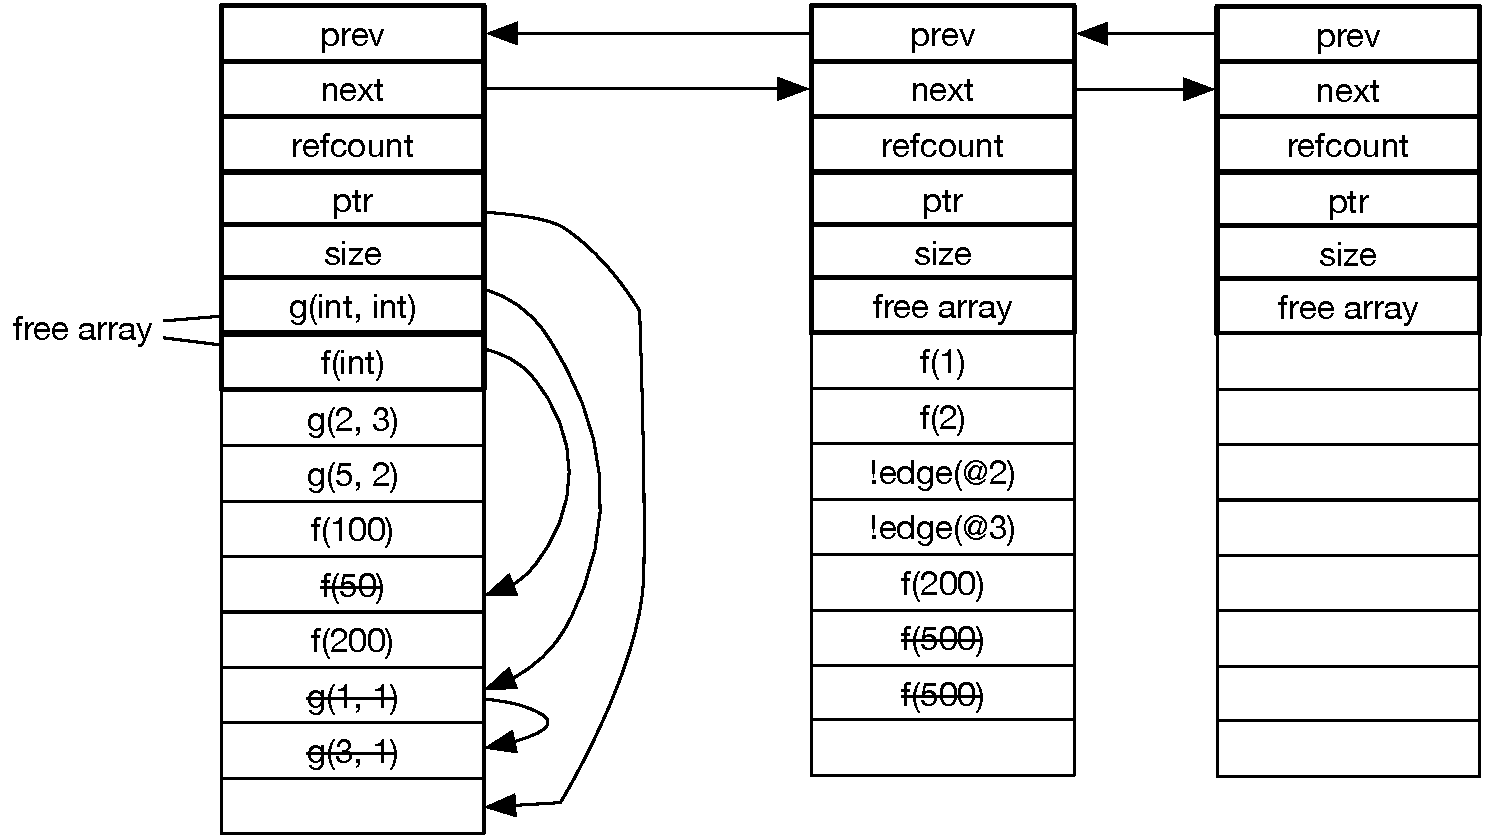
\includegraphics[width=0.7\linewidth]{figures/implementation/fact_allocator.pdf}
   \end{center}
   \caption{Fact allocator: each node has a pool of memory chunks for allocating
      logical facts. Each chunk contains: (1) several linked lists of free facts
      of the same size (\code{free\_list}); (2) a reference count of used facts
      (\code{refcount}); (3) a \code{ptr} pointer that points to unallocated
      space in the chunk. In this figure, predicates \code{f} and \code{g} have
   several deallocated facts that are ready to be used when a new fact needs to
be acquired.}
   \label{fig:implementation:fact_allocator}
\end{figure}
\fi


\section{Experimental Evaluation}
In this section, we evaluate the performance and scalability of the VM. The main
goals of this evaluation are as follows:

\begin{itemize}
   \item Compare the performance of LM programs against hand-written
      imperative C++ programs;
   \item Evaluate the scalability of said LM programs when using up to 20 cores
      concurrently;
   \item Understand the impact and effectiveness of our dynamic indexing
      algorithm and its indexing data structures used for logical facts (namely,
      hash tables);
   \item Understand the impact of the thread allocator and fact allocator on scalability and
      multicore performance;
\end{itemize}

For our experimental setup, we used a computer with a 24 (4x6) Core AMD
Opteron(tm) Processor 8425 HE $@$ 800 MHz with 64 GBytes of RAM memory running
the Linux Kernel 3.15.10-201.fc20.x86\_64. The C++ compiler used is the GCC
4.8.3 (g++) with the following \code{CXXFLAGS} flags: \code{-O3 -std=c++11
-march=x86-64}.  All experiments were executed 3 times and the running times
were averaged.

\subsection{Performance}

To understand the absolute performance of LM programs, we measured their
``sequential'' performance using a single thread of execution against
hand-written sequential C++ programs. All C++ programs were compiled with the
compilation flags that were used for LM in order to improve fairness. Arguably,
compiled C/C++ programs are a good standard for understanding the baseline
performance of new language runtimes, since compiled C/C++ programs tend to come
up on top on several popular programming language
benchmarks~\cite{language_benchmarks}.  Furthermore, the performance of
sequential C++ programs is a better baseline for measuring the scalability of LM
since these programs are sequential and thus provide a better baseline than the
``sequential'' run time of LM programs, which includes extra code for managing
synchronization between multiple (inexistent) threads.

In order to make our comparison more interesting, we also provide comparisons to
the Python language and other relevant systems. Python is a \emph{scripting}
programming language that is much slower than compiled C/C++ programs and thus
is a good upper-bound in terms of performance.

The goal of the evaluation is to understand the effectiveness of our compilation
strategy and the effectiveness of our dynamic indexing algorithms, including the
data structures (hash tables) which are used to store index logical facts. The
LM programs used in the experiments are the following:

\begin{itemize}
   \item Multiple Single Shortest Distance (MSSD): a program that computes the
      shortest distance from a subset of nodes of the graph to the all the nodes
      in the graph. A modified version is presented in
      Section~\ref{section:coord:rationale}.

      
    \item MiniMax: the AI algorithm for selecting the best player move in a
       Tic-Tac-Toe game. The initial board was augmented in order to provide a
       longer running benchmark. Program is presented in
       Section~\ref{section:coord:minimax}.

   \item Belief Propagation: a machine learning to denoise images. Program is
      explained in Section~\ref{sec:coordination:bp}.

    \item Heat Transfer: an asynchronous program that performs transfer of heat
       between nodes. Program is explained in Section~\ref{section:coord:ht}.

   \item N-Queens: the classic puzzle for placing queens on a chess board so
      that no two queens threaten each other. Program is explained in
      Section~\ref{section:coord:nqueens}.

\end{itemize}

Table~\ref{table:implementation:absolute} presents the comparison between LM and
sequential C++ programs. Comparisons to other systems are shown under the
\textbf{Other} column. Since we also want to assess the VM's scalability for
different program sizes, we use different datasets in several programs.

\begin{table}[ht]
   \begin{center}
      \begin{tabular}{c | c || c | c | c} \hline
	\textbf{Program} & \textbf{Size} & \textbf{C++ Time} (s) & \textbf{LM} & \textbf{Other} \\ \hline \hline
	\multirow{4}{*}{Belief Propagation}  & 50x50 &  3.16  &  1.27  &  1.08 (GraphLab) \\
		 & 200x200 &  49.36  &  1.36  &  1.25 (GraphLab) \\
		 & 300x300 &  135.56  &  1.35  &  1.25 (GraphLab) \\
		 & 400x400 &  169.99  &  1.35  &  1.27 (GraphLab) \\
	\hline
	\multirow{2}{*}{Heat Transfer}  & 80x80 &  4.62  &  7.28  &  - \\
		 & 120x120 &  20.29  &  7.07  &  - \\
	\hline
	\multirow{7}{*}{MSSD}  & US 500 Airports &  0.69  &  2.76  &  13.44 (Python) 0.25 (Ligra) \\
		 & OCLinks &  7.00  &  7.35  &  16.10 (Python) 0.34 (Ligra) \\
		 & EU Email &  13.47  &  2.08  &  9.80 (Python) 0.32 (Ligra) \\
		 & Twitter &  27.22  &  8.58  &  8.28 (Python) 0.27 (Ligra) \\
		 & US Power Grid &  55.33  &  5.64  &  10.99 (Python) 0.30 (Ligra) \\
		 & Live Journal &  221.91  &  4.38  &  0.20 (Ligra) \\
		 & Orkut &  281.59  &  1.66  &  4.23 (Python) 0.23 (Ligra) \\
	\hline
	\multirow{2}{*}{MiniMax}  & Small &  2.89  &  7.58  &  27.43 (Python) \\
		 & Big &  21.47  &  8.81  &  - \\
	\hline
	\multirow{4}{*}{N-Queens}  & 11 &  0.28  &  1.81  &  20.36 (Python) \\
		 & 12 &  1.42  &  3.09  &  24.30 (Python) \\
		 & 13 &  7.90  &  4.99  &  27.85 (Python) \\
		 & 14 &  47.90  &  6.42  &  31.52 (Python) \\
	\hline
\end{tabular}

   \end{center}

   \caption{Experimental results comparing different programs against
      hand-written versions in C++. For the C++ programs, we show the execution
      time in seconds (\textbf{C++ Time (s)}). For the other approaches, we show
      the overhead ratio compared with the corresponding C++ program. The
      overhead numbers (\textbf{lower is better}) are computed by dividing the
   execution time of the approach on that column by the execution time of the
similar hand-written C++ program.}

   \label{table:implementation:absolute}
\end{table}

For the MSSD program, we have used four datasets, which we describe as follows:

\begin{itemize}
   \item US 500 Airports~\cite{usairports,tnet}, a graph of the 500 top airports in the US with around
      5000 connections. The shortest distance is calculated for all nodes;
      
   \item OCLinks~\cite{tnet,oclinks}, a facebook-like social network with around 2000 nodes and 20000 edges. The shortest
      distance is calculated for 33\% of the nodes;

   \item US Power Grid~\cite{tnet,uspowergrid}, the power grid for western US with around 5000
      nodes and 13000 edges. The shortest distance is calculated for 20\% of the
      nodes;

   \item Email~\cite{snapnets}, a larger graph with 265000 nodes and 420000
      edges. The shortest distance was calculated for 100 nodes.

\end{itemize}

The C++'s MSSD programs applies the Dijkstra algorithm for each node we want to
compute the shortest distance from. While the Dijkstra algorithm has a better
complexity than the algorithm used in LM's algorithm, LM's algorithm is able to
process distances from multiple sources at the same time. Our experiments show
that the C++ program effectively beats LM's version by a large margin, but that
gap is reduced as the number of nodes increases. The C++ program needs to
initialize the Dijkstra algorithm for each source node, dropping its absolute
perform to just half of LM's performance. These results are also affected by the
increased locality and indexing used in LM's VM, which is shown to scale well in
our experiments. Python is much slower than LM but the gap between C++ is also
decreased as the graph gets larger.

The C++ version of the MiniMax program uses a single recursive function that
updates a single state as it is recursively called to generate the best score
and move. The LM version is seven times slower due to the costs of creating new
nodes using the exists construct and the large memory requirements as shown
next. In Chapter~\ref{chapter:coordination} we will show how to improve the the
space complexity of the MiniMax program and the corresponding run time.  Another
interesting aspect of the MiniMax program is that it does not use any persistent
predicate and therefore does not use array data structures for managing facts,
which have show to improve the run time of several programs in previous
experiments.

The Belief Propagation experiment is the program where LM performs the best when
compared to the C++ version. We found out that the mathematical operations
required to update the nodes belief values are expensive and make up a huge part
of the total computation time. This is clearly shown in the low overhead
numbers. We also compared our performance against the GraphLab and LM is only
slightly slower, which is also a point in LM's favour.

The Heat Transfer program behaves somewhat like Belief Propagation but LM is
almost an order of magnitude slower than the C++ version. We think this is
because the heat transfer computation is very small which tends to exacerbate
slower and repeated fact derivations on different nodes that are used to
propagate new heat values.

The LM's N-Queens programs shows some scalability issues since the overhead
ratio increases as the size of the problem increases. However, the same
behavior is seen in the Python program. The C++ program uses a backtracking
strategy to try out all the possibilities and uses a vector to store placements.
Since there is only at most $N$ (size of the board) vectors at the same time, it
shows better behavior than all the other programs. However, we should note that a
3-fold slowdown is a fairly good trade-off for a higher-level program that runs
faster than the C++ version when using 4 to 5 threads.

From these results, it is possible to conclude that LM's virtual machine offers
a decent performance when compared to hand-written C++ programs. We think these
results originate from four main aspects of our system: efficient indexing,
data structures with good locality such as array data structures for persistent
facts, improved memory locality from the memory allocator, and an efficient LM
to C++ compilation scheme. As noted in~\cite{cost}, scalability should not be
the sole focus of a parallel/distributed system such as LM. We have shown that
LM programs run reasonably fast and we will show next that they also scale well.

\subsubsection{Memory usage}

To complete our comparison against the C++ programs, we have measured and
compared the average memory used by both systems.
Table~\ref{table:implementation:mem} presents the memory statistics for LM
programs while Table~\ref{table:implementation:cmem} presents statistics for the
C++ programs.

\begin{table}[ht]
   \begin{center}
      \begin{tabular}{c | c || c | c | c || c c} \hline
	\textbf{Program} & \textbf{Size} & \textbf{Average} & \textbf{Final} & \textbf{Malloc} & \textbf{\# Facts} & \textbf{Each} \\ \hline \hline
	\multirow{4}{*}{Belief Propagation}  & 50x50 & 131MB & 264MB & 32 & 34K & 7.87KB \\
		 & 200x200 & 2GB & 4GB & 40 & 557K & 8.66KB \\
		 & 300x300 & 6GB & 12GB & 42 & 1256K & 10.43KB \\
		 & 400x400 & 7GB & 15GB & 43 & 2M & 7.47KB \\
	\hline
	\multirow{2}{*}{Heat Transfer}  & 80x80 & 8MB & 8MB & 20 & 63K & 0.14KB \\
		 & 120x120 & 18MB & 19MB & 22 & 143K & 0.14KB \\
	\hline
	\multirow{6}{*}{MSSD}  & US 500 Airports & 23MB & 15MB & 29 & 164K & 0.10KB \\
		 & OCLinks & 457MB & 216MB & 37 & 2M & 0.10KB \\
		 & EU Email & 449MB & 380MB & 38 & 3M & 0.13KB \\
		 & Twitter & 895MB & 332MB & 47 & 4M & 0.08KB \\
		 & US Power Grid & 1827MB & 2GB & 41 & 24M & 0.10KB \\
		 & Orkut & 3GB & 2GB & 60 & 100M & 0.03KB \\
	\hline
	\multirow{2}{*}{MiniMax}  & Small & 1794MB & 33KB & 42 & 2 & 16.50KB \\
		 & Big & 14GB & 33KB & 48 & 2 & 16.50KB \\
	\hline
	\multirow{4}{*}{N-Queens}  & 11 & 1282KB & 673KB & 29 & 3K & 0.20KB \\
		 & 12 & 4MB & 2MB & 34 & 14K & 0.20KB \\
		 & 13 & 20MB & 14MB & 38 & 74K & 0.20KB \\
		 & 14 & 95MB & 73MB & 43 & 366K & 0.20KB \\
	\hline
\end{tabular}

   \end{center}
   \caption{Memory statistics for LM programs. The meaning of each column is as
      follows: column \textbf{Average} represents the average memory use of the
      program; \textbf{Final} represents the memory usage after the program
      completes; \textbf{Malloc} represents the number of \code{malloc}
   operations requested to the operating system by the VM's memory allocator;
   \textbf{\# Facts} represents the number of facts in the database after the
   program completes; \textbf{Each} is the result of dividing \textbf{Final} by
   \textbf{\# Facts} and represents the average memory required per fact.}
   \label{table:implementation:mem}
\end{table}

The MSSD program shows that LM's VM requires 2 to 5 times more memory than the
corresponding C++ program. The ratio is larger when the dataset used is smaller
which is understandable due to the extra data structures required by the VM
(namely the node data structure). In terms of average memory per fact, we see
that the MSSD requires on average 60B, which is not bad considering that, in
reality, each fact for this particular program requires around 32B. This
indicates that all those extra data structures represent a relatively minor
overhead.

\begin{table}[ht]
   \begin{center}
      \begin{tabular}{c | c | c | c} \hline
	\textbf{Program} & \textbf{Size} & \textbf{Average} & \textbf{Final} \\ \hline \hline
	\multirow{4}{*}{Belief Propagation}  & 50x50 & 2.7MB & 2.7MB\\
		 & 200x200 & 45.1MB & 45.1MB\\
		 & 300x300 & 99.7MB & 99.8MB\\
		 & 400x400 & 181.3MB & 181.4MB\\
	\hline
	\multirow{2}{*}{Heat Transfer}  & 80x80 & 2.3MB & 2.3MB\\
		 & 120x120 & 5.4MB & 5.4MB\\
	\hline
	\multirow{7}{*}{MSSD}  & US 500 Airports & 7.8MB & 15.7MB\\
		 & OCLinks & 76.6MB & 151.9MB\\
		 & EU Email & 267.3MB & 298.2MB\\
		 & Twitter & 245.3MB & 333.10MB\\
		 & US Power Grid & 744.5MB & 1491.7MB\\
		 & Live Journal & 5.4GB & 5.4GB\\
		 & Orkut & 7.5GB & 7.6GB\\
	\hline
	\multirow{2}{*}{MiniMax}  & Small & 1KB & 0KB\\
		 & Big & 1KB & 0KB\\
	\hline
\end{tabular}

   \end{center}
   \caption{Average memory usage of each C++ program.}
   \label{table:implementation:cmem}
\end{table}


When the MiniMax program completes, there is only a single fact on the database
that indicates the best player move. The MiniMax program is also the only
program in this experiment that dynamically generates a (tree) graph, which is
destroyed once the best move is found. The garbage collector implemented the VM
that collects empty nodes, is able to delete all those nodes since the
\textbf{Final} memory usage is much smaller than the \textbf{Average} statistic.
However, because the garbage collector retains a small number of freed nodes
that may be reused later, the average size per fact is 15.50KB, which also
includes those freed nodes. Finally, the memory usage of the C++ program is much
better because the C++ program uses function calls to represent the tree
structure of the MiniMax algorithm.

The Belief Propagation program shows that LM's VM has a much higher resource
usage than the corresponding C++ version. This is because the nodes in the LM's
program keep a copy of the belief values of neighbor nodes, while the C++
program performs uses shared memory and the stack to read and compute the
neighbors belief values. Interestingly, this issue does not happen in the Heat
Transfer program, where heat values are shared between nodes, reducing the need
to keep facts with unique lists around. Notably, the C++ memory usage is not
much smaller than LM's VM.

Finally, for the N-Queens program it is possible to immediately understand whey
there may be scalability issues when using larger data sets because the memory
usage increases significantly when using larger boards. On the positive side,
the average memory usage per fact remains the same for all data sets. In respect
to the C++ program, it is expected that it should consume almost no memory
because it uses the stack to compute the problem solutions.

\subsubsection{Indexing and data structures}

We now evaluate the impact of our dynamic indexing algorithm and related data
structures. For this, we have rerun the previous experiments and compared the
results against the optimized version.
Table~\ref{table:implementation:compare_absolute} shows the comparison between
the optimized version of the VM and the version of the VM with indexing
disabled. From column \textbf{Run Time} shows that the MSSD program benefits
from indexing because the unoptimized version is around 25 to 75 times slower
than the version with indexing enabled. Since MSSD computes the shortest
distance to multiple nodes, its rules require searching for the shortest
distance facts of arbitrary nodes. All the other programs do not require index
but also do not display any significant slowdown from using dynamic indexing. In
terms of memory usage, the version with indexing uses slightly more memory,
especially for MSSD program, where the US Power Grid dataset requires 50\% more
memory due to the existence of hash tables used for supporting indexing.

\begin{table}[ht]
   \begin{center}
      \begin{tabular}{c | c || c | c} \hline
	\textbf{Program} & \textbf{Size} & \textbf{Run Time} & \textbf{Average Memory}\\ \hline \hline
	\multirow{4}{*}{Belief Propagation}  & 50x50 &  0.88  &  1.00
  \\
		 & 200x200 &  1.00  &  1.00
  \\
		 & 300x300 &  1.08  &  1.00
  \\
		 & 400x400 &  1.01  &  1.00
  \\
	\hline
	\multirow{2}{*}{Heat Transfer}  & 80x80 &  1.01  &  1.00
  \\
		 & 120x120 &  1.12  &  1.00
  \\
	\hline
	\multirow{4}{*}{MSSD}  & US 500 Airports &  34.57  &  1.65
  \\
		 & OCLinks &  108.93  &  1.36
  \\
		 & EU Email &  3.86  &  1.45
  \\
		 & Twitter &  1.97  &  1.19
  \\
	\hline
	\multirow{2}{*}{MiniMax}  & Small &  0.98  &  1.00
  \\
		 & Big &  0.95  &  1.00
  \\
	\hline
	\multirow{4}{*}{N-Queens}  & 11 &  0.98  &  1.00
  \\
		 & 12 &  1.00  &  1.00
  \\
		 & 13 &  1.00  &  1.00
  \\
		 & 14 &  1.00  &  1.00
  \\
	\hline
\end{tabular}

   \end{center}
   \caption{Measuring the impact of dynamic indexing and related database data
      structures. Column \textbf{Run Time} shows the slow down ratio of the
      unoptimized version (numbers greater than 1 show indexing improvements).
      Column \textbf{Average Memory} is the result of dividing the average
      memory of the optimized version by the unoptimized version (large numbers
      indicate that more memory is needed when using indexing mechanisms).}
   \label{table:implementation:compare_absolute}
\end{table}

\subsubsection{Array data structures}

Another important implementation detail is the use of array data structures for
storing persistent facts that are not derived by rule derivation but only exist
as initial facts. These cases are detected by the compiler and allow the VM to
improve memory locality and reduce memory usage by packing persistent facts in a
contiguous memory area.

\begin{table}[ht]
   \begin{center}
      \begin{tabular}{c | c || c | c} \hline
	\textbf{Program} & \textbf{Size} & \textbf{Run Time} & \textbf{Average Memory}\\ \hline \hline
	\multirow{4}{*}{Belief Propagation}  & 50x50 &  0.94  &  0.99
  \\
		 & 200x200 &  1.03  &  0.99
  \\
		 & 300x300 &  1.02  &  0.99
  \\
		 & 400x400 &  1.05  &  0.99
  \\
	\hline
	\multirow{2}{*}{Heat Transfer}  & 80x80 &  1.17  &  0.62
  \\
		 & 120x120 &  1.19  &  0.62
  \\
	\hline
	\multirow{4}{*}{MSSD}  & US 500 Airports &  1.64  &  0.65
  \\
		 & OCLinks &  0.31  &  3.23
  \\
		 & EU Email &  0.68  &  0.95
  \\
		 & US Power Grid &  0.08  &  8.27
  \\
	\hline
	MiniMax  & Small &  0.98  &  1.01
  \\
	\hline
	\multirow{4}{*}{N-Queens}  & 11 &  0.85  &  0.94
  \\
		 & 12 &  0.71  &  0.98
  \\
		 & 13 &  0.58  &  0.99
  \\
		 & 14 &  0.55  &  1.00
  \\
	\hline
\end{tabular}

   \end{center}

   \caption{Measuring the impact of using array data structures for persistent
      facts. Column \textbf{Run Time} shows the speedups obtained by using
      arrays. Column \textbf{Average Memory} is the result of dividing the
      average memory of the programs using arrays by the version without them
      (e.g., numbers show memory usage reduction when using array data
   structures).}

   \label{table:implementation:compare_arrays}
\end{table}

I think we should remove this stuff XXX

\subsection{Scalability}
In this section, we analyze the scalability of several LM programs using up to
32 threads. Note that we are studying declarative LM programs that do not make
use of coordination. We also compare the run times against the run time of the
hand-written C++ programs when such run times are available. We used the
programs of the previous section with a few additions:

\begin{itemize}
      \item PageRank: an asynchronous version of the PageRank program without
         synchronization between iterations. Every time a node sends a new
         PageRank value to its neighbors and the change is significant, then the
         neighbors are scheduled to recompute their PageRanks.

      \item Greedy Graph Coloring~(GGC): an algorithm that colors nodes in a
         graph so that no two adjacent nodes have the same color. We start with
         a small number of colors and then we expand the number of colors when
         we cannot color the graph.

\end{itemize}

These two programs were not used in the previous section because we did not
implement the corresponding C++ program.

We executed all the programs using 17 configurations. The base configuration
uses 1 thread and the other 16 configurations use an even numbers of threads for
a maximum of 32 threads. Figure~\ref{fig:evaluation:overview} presents the
overall scalability computed as the weighted harmonic mean of all the benchmarks
presented in this section. The weight used in the harmonic mean formula is the
run time of each program when executed with one thread. The one threaded version
executes with all the synchronization mechanisms enabled, just like the
multi-threaded executions. The experimental results show that, on average, our
benchmarks have a 15-fold speedup when using 32 threads.

\begin{figure}[]
        \centering
        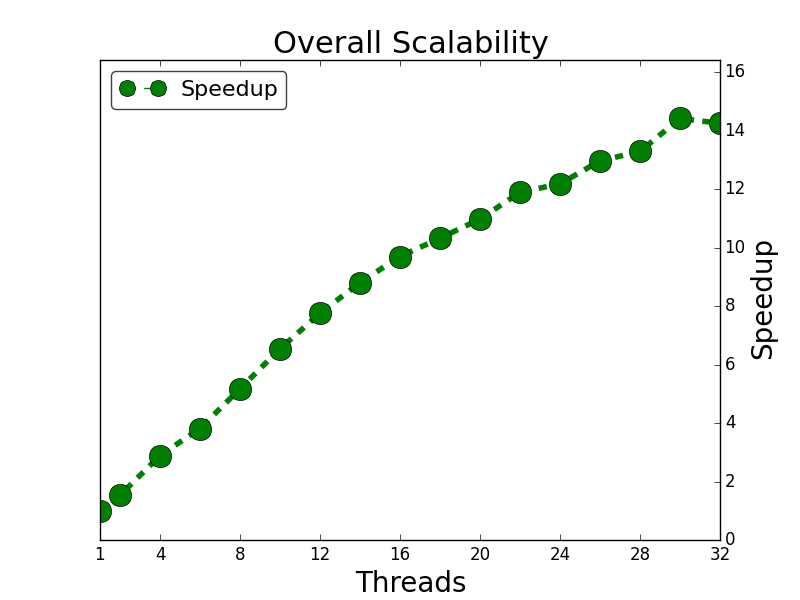
\includegraphics[width=\plotsize\textwidth]{experiments/scalability/overview.png}
        \mycap{Overall scalability for the benchmarks presented in this section.
        The average speedup is the weighted harmonic mean using the single threaded
     run time as the weight of each benchmark.}
        \label{fig:evaluation:overview}
\end{figure}


We now analyze each program separately. For the plots presented next, the $x$
axis represents the number of threads used, the left $y$ axis represents the run
time (in milliseconds) for that particular configuration and uses a logarithmic
scale and the right axis $y$ represents the speedup computed as $T_1/T_i$, where
$T_i$ represents the run time of the program using $i$ threads.  In some plots,
there is also an horizontal black line that represents the run time of the C++
program and is used to understand how many threads are needed in order for an LM
program to run faster than the C++ program. Note that all run times are the
average of three runs.

The scalability results for the Belief Propagation program are presented in
Fig.~\ref{fig:implementation:scale_bp}. This program has the best scalability
with a 60-fold speedup for 32 threads. This is because the default ordering used
for 1 thread is not optimal, while the same ordering works better for multiple
threads. Additionally, the existence of multiple threads increase the amount of
up-to-date information from neighbor nodes, resulting in super-linear speedups.
Note that we also used the same computation ordering in the C++ program, which
is also the one used in the GraphLab framework.

\begin{figure}[]
        \centering
        \begin{subfigure}[b]{\plotsize\textwidth}
                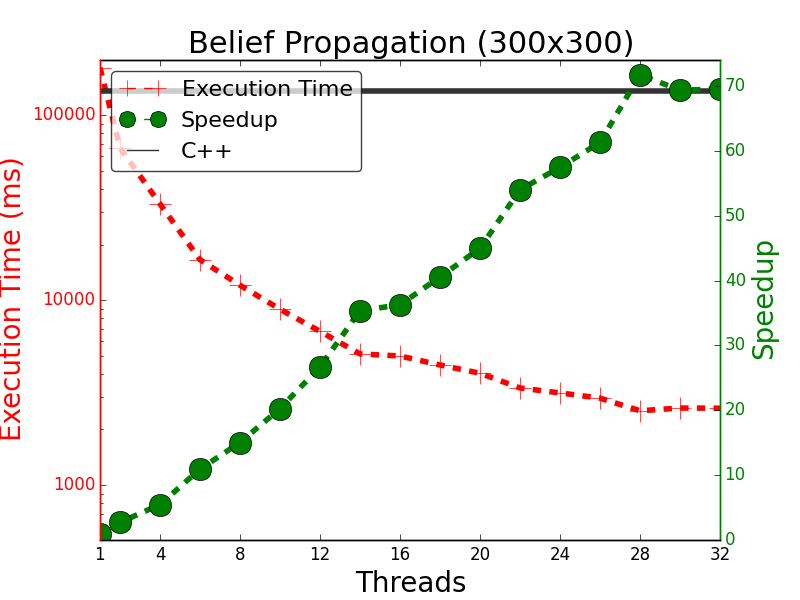
\includegraphics[width=\textwidth]{experiments/scalability/scale-belief-propagation-300.png}
                \label{fig:implementation:scale_bp300}
        \end{subfigure}
        ~
        \begin{subfigure}[b]{\plotsize\textwidth}
                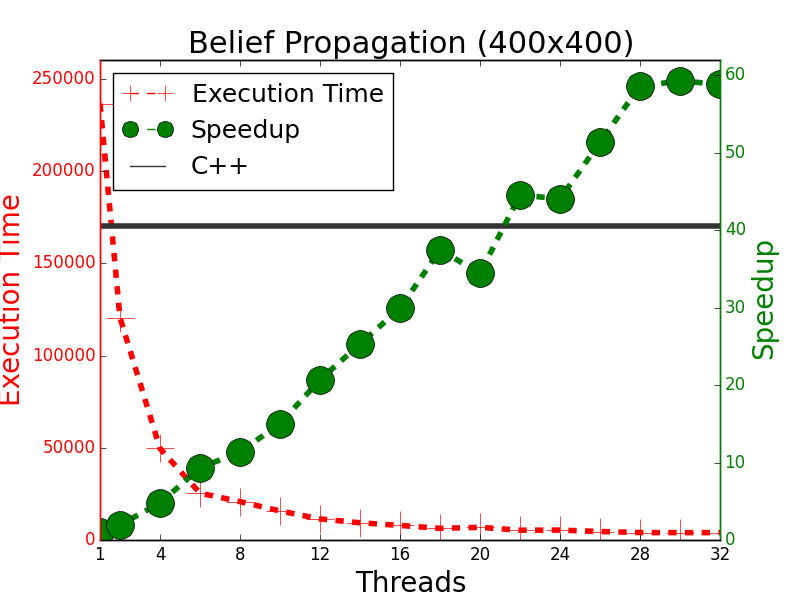
\includegraphics[width=\textwidth]{experiments/scalability/scale-belief-propagation-400.png}
                \label{fig:implementation:scale_bp400}
        \end{subfigure}\\
        \mycap{Scalability results of the Belief Propagation program.}
        \label{fig:implementation:scale_bp}
\end{figure}

The results for the Heat Transfer program are shown in
Fig.~\ref{fig:implementation:scale_ht}. We note that LM requires around 15
threads to reach the run time of the C++ program. This results from the poor
absolute performance of the LM program that was mentioned in the previous section.
Although we use a grid dataset, the work available in the graph is not equally
distributed due to different initial heat values, therefore an almost linear
speedup should not be expected. When comparing the two datasets used, the 80x80
configuration has less scalability than the 120x120 dataset due to its smaller
size. For the 120x120 dataset, LM has a 12-fold speedup for 32 threads, which
makes the LM version run almost twice as fast as the C++ version.

\begin{figure}[]
        \begin{subfigure}[b]{\plotsize\textwidth}
                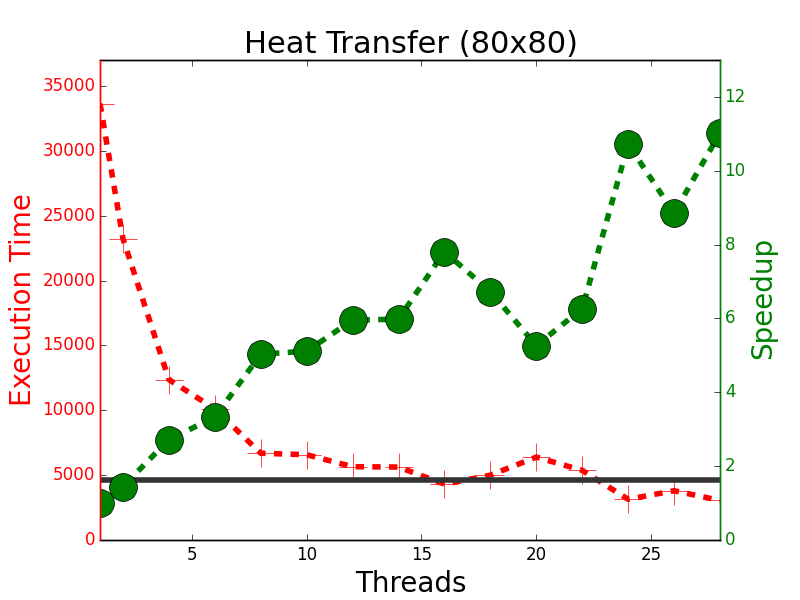
\includegraphics[width=\textwidth]{experiments/scalability/scale-new-heat-transfer-80.png}
                \label{fig:implementation:scale_ht80}
        \end{subfigure}
        ~
        \begin{subfigure}[b]{\plotsize\textwidth}
                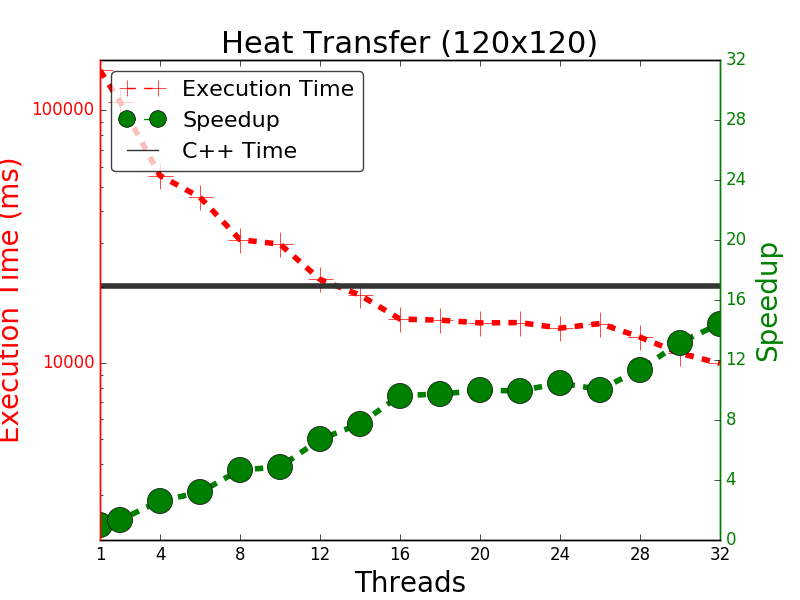
\includegraphics[width=\textwidth]{experiments/scalability/scale-new-heat-transfer-120.png}
                \label{fig:implementation:scale_ht120}
        \end{subfigure}\\
        \mycap{Scalability results for the Heat Transfer program. Because the
           Heat Transfer program performs poorly when compared to the C++ program,
           the LM version needs at least 15 threads to reach the run time of the C++
           program (for the 120x120 dataset).}
        \label{fig:implementation:scale_ht}
\end{figure}

Figure~\ref{fig:implementation:scale_ggc} presents the results for the Greedy
Graph Coloring~(GGC) program. In GGC, we use two datasets: Google
Plus~\cite{snapnets}, a graph representing social circles in Google Plus with
107614 nodes and 13673453 edges, and Twitter, a graph representing Twitter
networks with 81306 nodes and 1768149 edges (note that Twitter was also used
before in the MSSD program). The Twitter and Google Plus datasets have almost
the same number of nodes but Google Plus has ten times more edges, which makes
coloring more time consuming. Since Twitter is a much smaller dataset, its
speedup is much smaller than Google Plus, as expected. However, while the
speedup of Twitter starts to drop after 16 threads, the LM system is still able
to make it faster by adding more threads. For Google Plus, a 20-fold speedup is
achieved for 32 threads, which is a reasonable scalability considering that GGC
is not a program where work is equally distributed.

\begin{figure}[]
        \begin{subfigure}[b]{\plotsize\textwidth}
                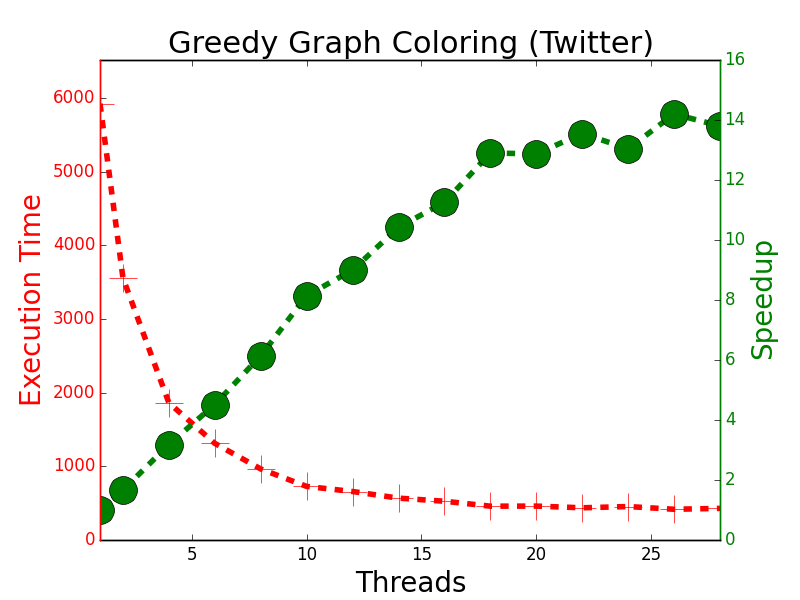
\includegraphics[width=\textwidth]{experiments/scalability/scale-greedy-graph-coloring-twitter.png}
                \label{fig:implementation:scale_ggc_twitter}
        \end{subfigure}
        ~
        \begin{subfigure}[b]{\plotsize\textwidth}
                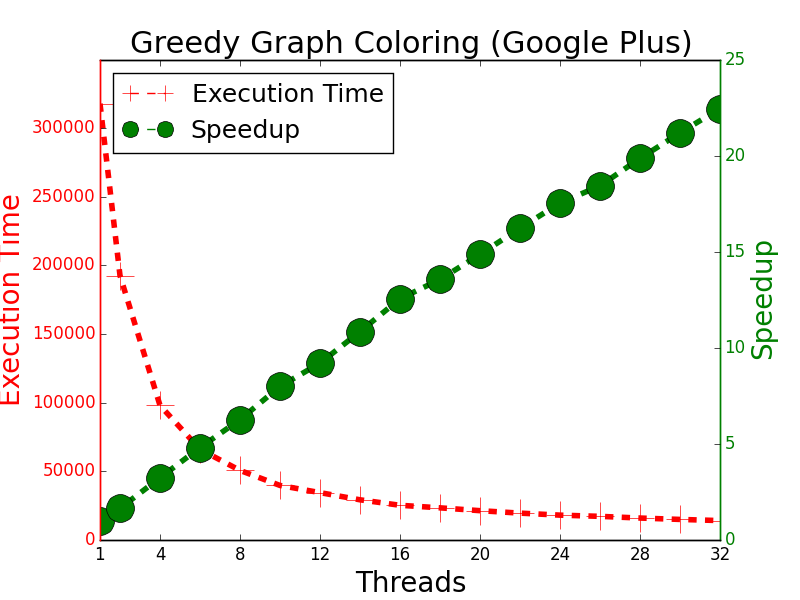
\includegraphics[width=\textwidth]{experiments/scalability/scale-greedy-graph-coloring-gplus.png}
                \label{fig:implementation:scale_ggc_gplus}
        \end{subfigure}\\

        \mycap{Scalability of the Greedy Graph Coloring program.}

        \label{fig:implementation:scale_ggc}
\end{figure}

The results for the N-Queens program are shown in
Fig.~\ref{fig:implementation:scale_queens}. We decided to just use the 13 and 14
configurations since those take longer to run. The 13-Queens configuration has
169 (13x13) nodes while the 14-Queens configuration has 196 (14x14) nodes. The LM program
considers the chess board as a graph and the bottom rows have more work to
perform since the valid queens placements are built from the top to the bottom
row. For a more in-depth explanation of the N-Queens program please see
Section~\ref{section:coord:nqueens}.

Due to the small number of nodes in the N-Queens program and the fact that more
work is performed at the bottom rows, the N-Queens program is hard to
parallelize. Furthermore, the solutions for the puzzle are built by constructing
lists which are shared between threads. This introduces some potential false
sharing because the reference count of each list data structure needs to be
updated when new solutions are constructed. The 14-Queens configuration has good
efficiency using 16 to 20 threads, while the 13-Queens configuration efficiency
starts to drop after 14 threads. One can argue that the best number of threads
is correlated to the size of the board, because the second half of execution is
better balanced and partitioned when the number of threads matches the size of
the board.

\begin{figure}[]
        \centering
        \begin{subfigure}[b]{\plotsize\textwidth}
                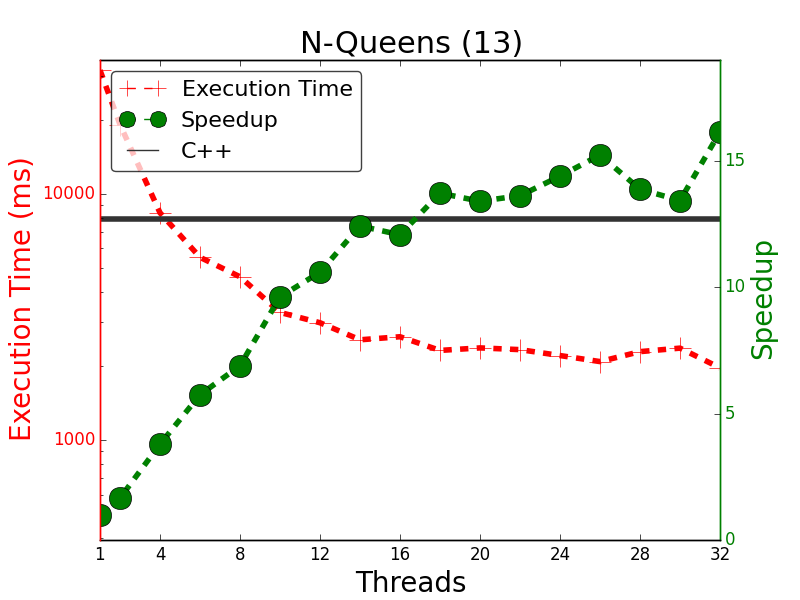
\includegraphics[width=\textwidth]{experiments/scalability/scale-8queens-13.png}
                \label{fig:implementation:scale_queens13}
        \end{subfigure}
        ~
        \begin{subfigure}[b]{\plotsize\textwidth}
                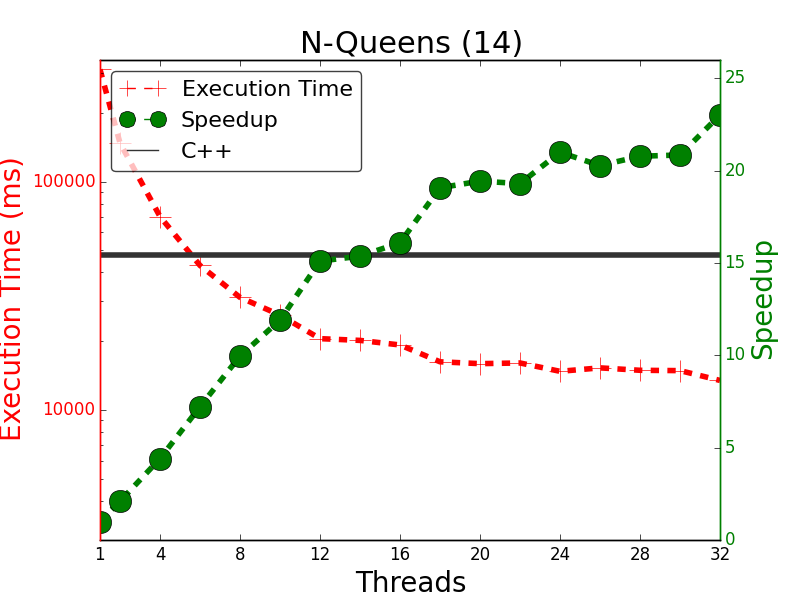
\includegraphics[width=\textwidth]{experiments/scalability/scale-8queens-14.png}
                \label{fig:implementation:scale_queens14}
        \end{subfigure}

        \mycap{Scalability results for the N-Queens program. The 13
        configuration has 73712 solutions, while the 14 configuration has 365596
     solutions. In terms of graph size, the 13 configuration has $13 \times 13$
  nodes while the 14 configuration has $14 \times 14$ nodes.}

        \label{fig:implementation:scale_queens}
\end{figure}

The speedup results for the MiniMax program is shown in
Fig.~\ref{fig:implementation:scale_minmax}.  This is an interesting program
because the graph is constructed during run time. Furthermore, due to the LM
default scheduling order, the tree is explored in a breadth-first fashion,
requiring the program to hold the complete MiniMax tree in memory. The Big
configuration, for instance, uses, on average, 14GB of memory and a total of
30GB of memory before collecting the tree. Since the machine used for the
experiments has only 32GB, the Small configuration scales better due to the
smaller memory requirements. In Section~\ref{section:coord:minimax}, we will
show how this program can be improved by changing the default scheduling order
of LM and improving the memory usage of the program.

\begin{figure}[]
        \begin{subfigure}[b]{\plotsize\textwidth}
                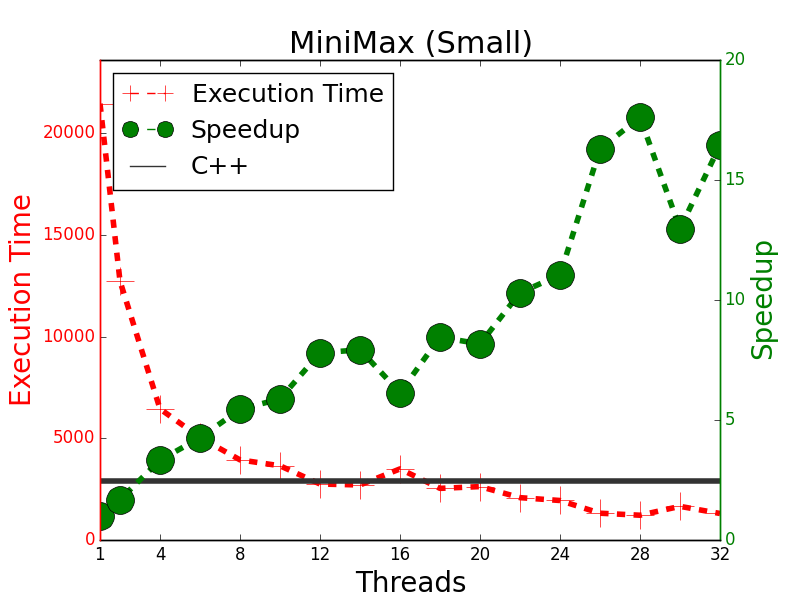
\includegraphics[width=\textwidth]{experiments/scalability/scale-min-max-tictactoe-small.png}
                \label{fig:implementation:scale_minmax_small}
        \end{subfigure}
        ~
        \begin{subfigure}[b]{\plotsize\textwidth}
                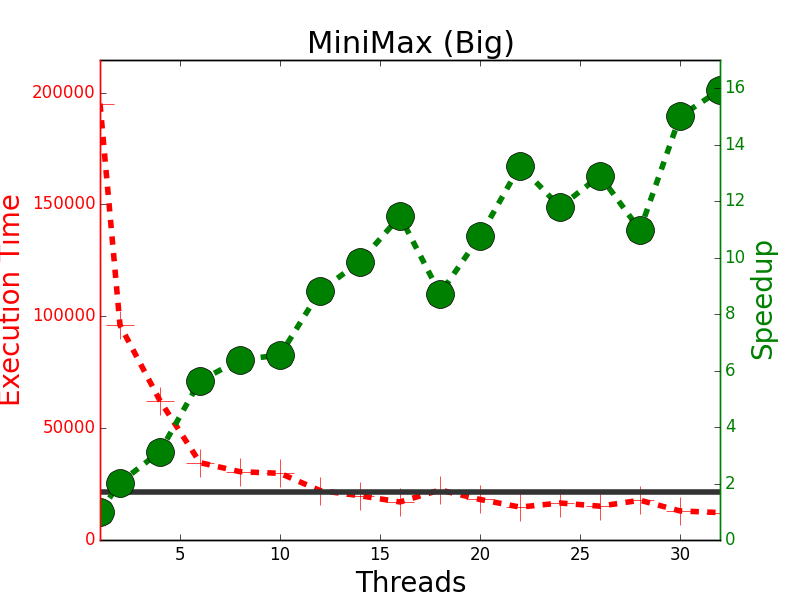
\includegraphics[width=\textwidth]{experiments/scalability/scale-min-max-tictactoe-big.png}
                \label{fig:implementation:scale_minmax_big}
        \end{subfigure}\\

        \mycap{Scalability for the MiniMax program. Although the Big
           configuration has more work available and could in principle scale
           better than Small, the high memory requirements of Big makes it scale
           poorly.}

        \label{fig:implementation:scale_minmax}
\end{figure}

The scalability results for the MSSD program are shown in
Fig.~\ref{fig:implementation:scale_sssp}. The amount of work required to compute
the results of each dataset depends on the size of the graph and the number of
nodes from which the distance must be computed. The first conclusion is that
more work implies more scalability, and the US Power Grid dataset has a 20-fold
speedup for 32 threads, the best from the 6 datasets used. The second conclusion
is that all datasets are able to, at least, reach the execution speed of the
corresponding C++ program. However, some datasets such as EU Email or Orkut, are
notoriously faster than C++ when using more than 5 threads, which is a
impressive result.  We think this is because the number of source nodes is
small. Furthermore, LM as a slight advantage over the C++ program because, in
LM, distances to different nodes are propagated at once, while in the C++
version, the Dijkstra algorithm runs in iterations - one for each node from
which we want to calculate the distance from.

\begin{figure}[]
        \centering
        \begin{subfigure}[b]{\plotsize\textwidth}
                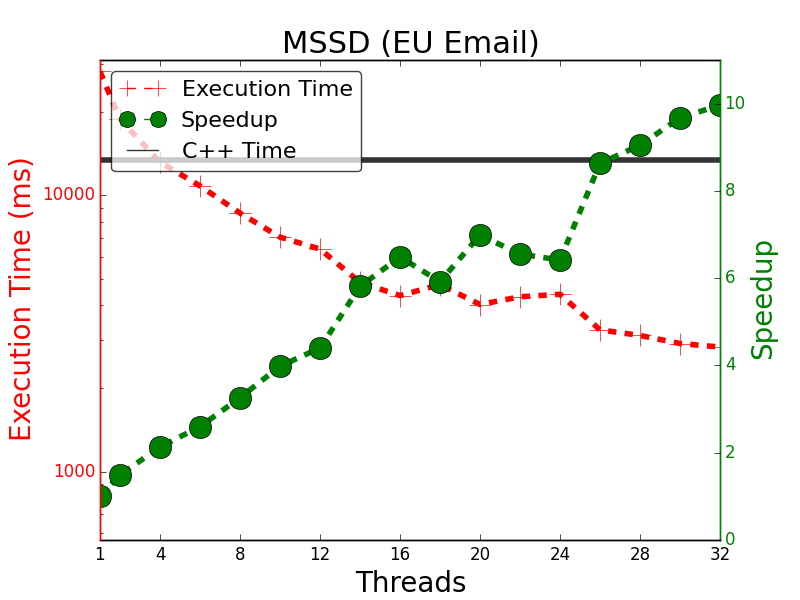
\includegraphics[width=\textwidth]{experiments/scalability/scale-shortest-email.png}
                \label{fig:implementation:scale_sssp_email}
                \mycap{Graph with 265000 nodes and 420000 edges. The shortest
                distance is calculated for 100 nodes.}
        \end{subfigure}
        ~
        \begin{subfigure}[b]{\plotsize\textwidth}
                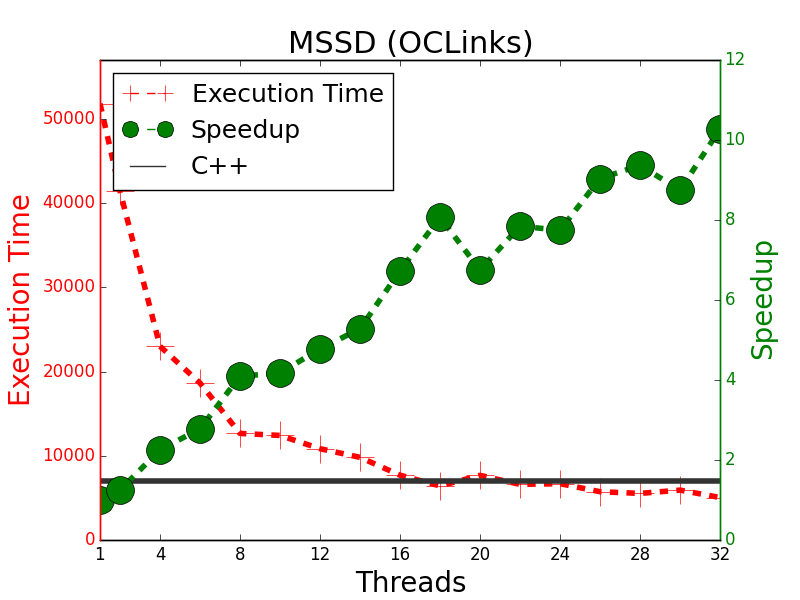
\includegraphics[width=\textwidth]{experiments/scalability/scale-shortest-oclinks.png}
                \label{fig:implementation:scale_sssp_oclinks}
                \mycap{Graph with around 2000 nodes and 20000 edges. The shortest
                   distance is calculated for all nodes.}
        \end{subfigure} \\
        \begin{subfigure}[b]{\plotsize\textwidth}
                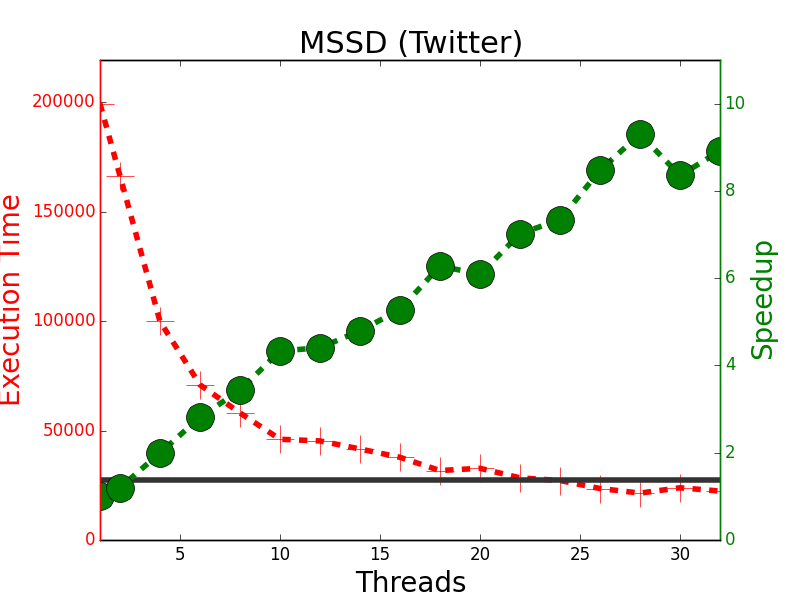
\includegraphics[width=\textwidth]{experiments/scalability/scale-shortest-twitter.png}
                \label{fig:implementation:scale_sssp_twitter}
                \mycap{Graph with 81306 nodes and 1768149 edges. The shortest
                   distance is calculated for 40 nodes.}
        \end{subfigure}
        ~
        \begin{subfigure}[b]{\plotsize\textwidth}
                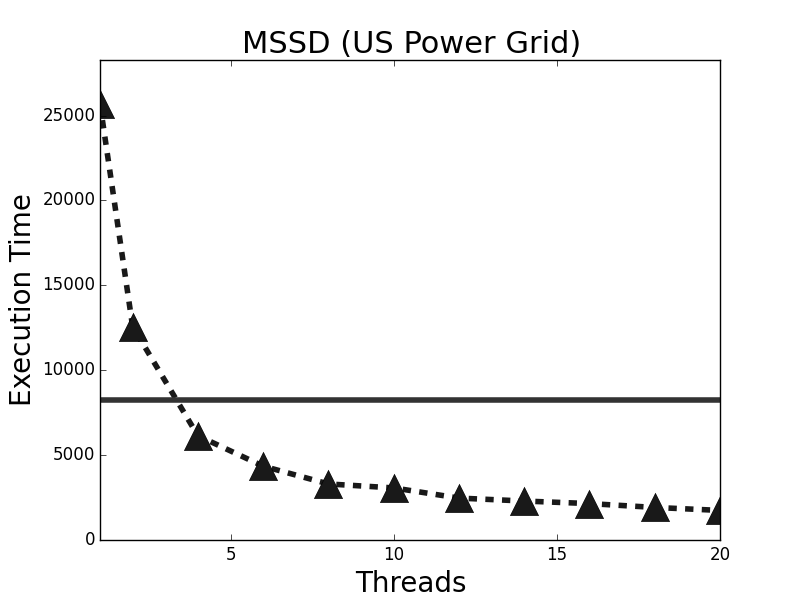
\includegraphics[width=\textwidth]{experiments/scalability/scale-shortest-uspowergrid.png}
                \label{fig:implementation:scale_sssp_uspowergrid}
                \mycap{Graph with around 5000 nodes and 13000 edges. The
                shortest distance is calculated for all nodes.}
        \end{subfigure}\\
        \begin{subfigure}[b]{\plotsize\textwidth}
                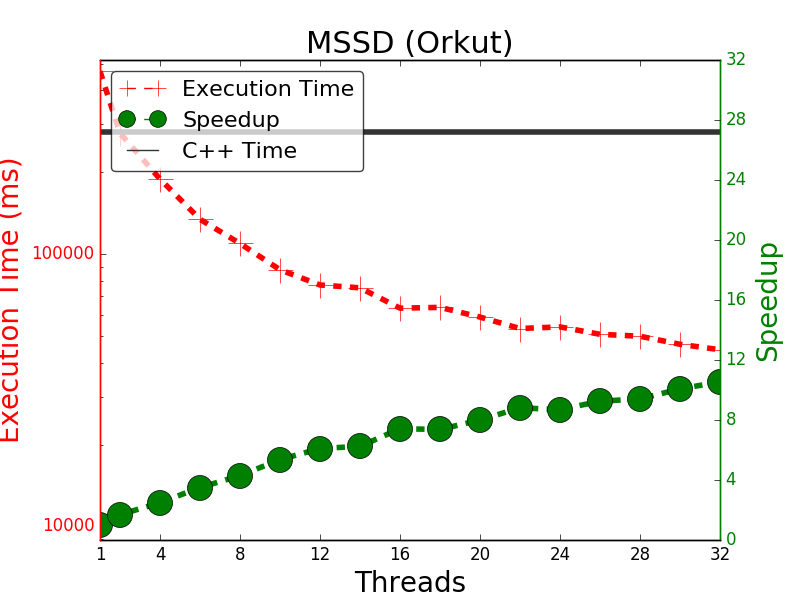
\includegraphics[width=\textwidth]{experiments/scalability/scale-shortest-orkut.png}
                \label{fig:implementation:scale_sssp_orkut}
                \mycap{Graph with 3072441 nodes and 117185083 edges. The shortest
                   distance is calculated for two nodes.}
        \end{subfigure}
        ~
        \begin{subfigure}[b]{\plotsize\textwidth}
                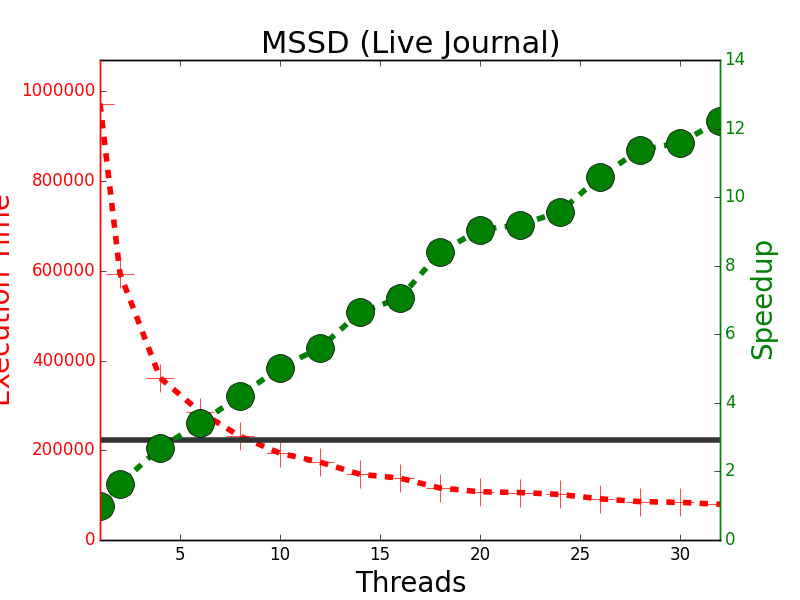
\includegraphics[width=\textwidth]{experiments/scalability/scale-shortest-livejournal.png}
                \label{fig:implementation:scale_sssp_livejournal}
                \mycap{Graph with around 4847571 nodes and 68993773 edges. The
                shortest distance is calculated for two nodes.}
        \end{subfigure}\\

        \mycap{Scalability for the MSSD program. The LM system scales better
        when there is more work to do per node, with the US Power Grid dataset
        showing the most scalability.}

        \label{fig:implementation:scale_sssp}
\end{figure}

The final scalability results are shown for PageRank in
Fig.~\ref{fig:implementation:scale_pagerank}. We used two datasets, Google Plus
and Pokec. Google Plus~\cite{snapnets} has 107614 nodes and 13673453 edges and is based on a Google Plus social network, while Pokec~\cite{snapnets} has
1632803 nodes and 30622564 edges and represents data from a popular social network website in Slovakia.
Even though Pokec is the larger graph, Google
Plus has a denser graph, where the average number of edges per node is 127
compared to the average of 18 for Pokec. This may explain why Google Plus is
more scalable with a 14-fold speedup for 32 threads.

\begin{figure}[]
        \begin{subfigure}[b]{\plotsize\textwidth}
                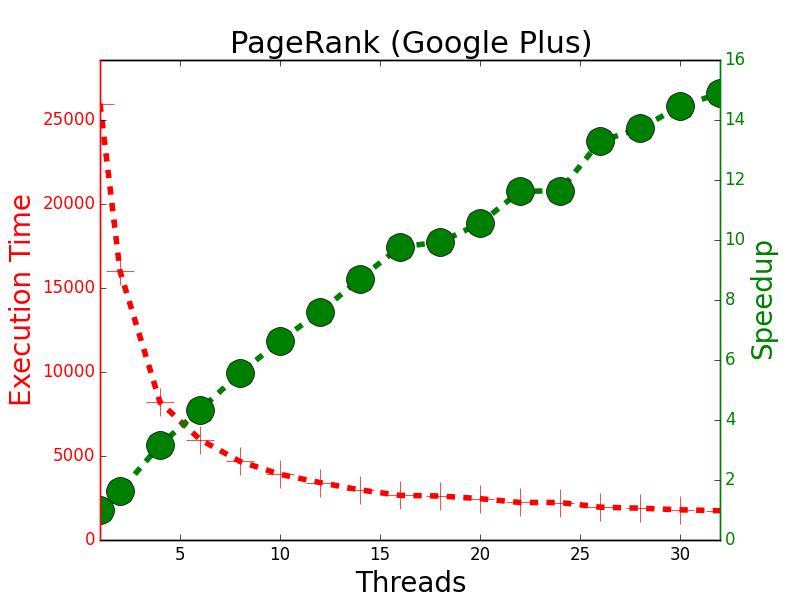
\includegraphics[width=\textwidth]{experiments/scalability/scale-pagerank-gplus.png}
                \label{fig:implementation:scale_pagerank_gplus}
                \mycap{The Google Plus graph has a high average of edges per
                node of 127.}
        \end{subfigure}
        ~
        \begin{subfigure}[b]{\plotsize\textwidth}
                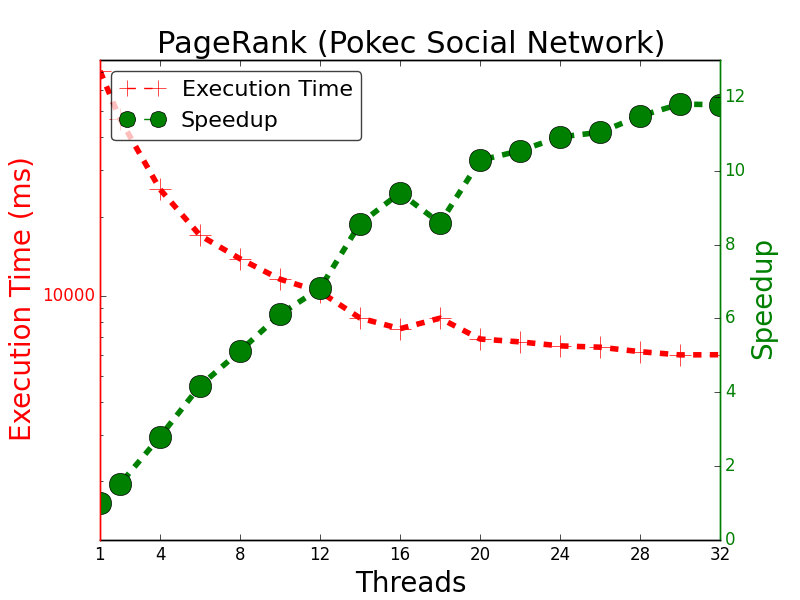
\includegraphics[width=\textwidth]{experiments/scalability/scale-pagerank-pokec.png}
                \label{fig:implementation:scale_pagerank_pokec}
                \mycap{The Pokec graph has a lower average of edges per node
                of 18.}
        \end{subfigure}\\
        \mycap{Scalability results for the asynchronous PageRank program. The
           superior scalability of the Google Plus dataset may be explained by
        its higher density of edges.}
        \label{fig:implementation:scale_pagerank}
\end{figure}


\subsubsection{Thread allocator evaluation}



\section{Related Work}
\paragraph{Virtual Machines}

Virtual machines are a popular technique for implementing interpreters for high
level programming languages. Due to the increased availability of parallel
and distributed architectures, several machines have been developed with
parallelism in mind~\cite{Kara:1997:AMM:265274}. One good example is
the Parallel Virtual Machine~(PVM)~\cite{Sunderam90pvm:a}, which servers as an
abstraction to program heterogeneous computers as a single machine. Another
important machine is the Threaded Abstract
Machine~(TAM)~\cite{CullerGSvE93,goldstein-tr94}, which defines a self-scheduled
machine language of parallel threads where a program is represented using
conventional control flow.

Prolog, the most prominent logic programming language, has a rich history of
virtual machine research centered extending/adapting the Warren Abstract
Machine~(WAM)~\cite{AICPub641:1983}.  Because Prolog programs tend to be
naturally parallel, much research has been done to either parallelize the WAM or
create new parallel machines. Two types of parallelism are possible in Prolog:
\emph{OR-parallelism}, where several clauses for the same goal can be executed,
and \emph{AND-parallelism}, where goals in the same clause are tried in
parallel. For OR-parallelism, we have several models such as: the SRI
model~\cite{Warren:1987:OEM:67683.67699}, the Argonne
model~\cite{ButlerDLOOS88}, the MUSE model~\cite{Ali:1990fk} and the BC
machine~\cite{Ali88}. For AND-parallelism, different implementations were built
on top of the WAM~\cite{Hermenegildo:1986:AMB:913061,Lin:1988:AEL:900478},
however more general models such as the Andorra
model~\cite{Haridi:1990:KAP:87961.87964} were developed which allows both AND
and OR-parallelism.

\paragraph{Datalog Execution} The Datalog language is a forwards-chaining logic
programming and therefore requires different evaluation strategies than those
used by Prolog, which is a backwards-chaining logic programming language.
Arguably, the most well-known strategy for Datalog programs with recursive rules
is the \emph{Semi-Na\"{\i}ve Fixpoint}
algorithm~\cite{Balbin:1987:GDA:34657.34661}, where the computation is split
into iterations and the facts generated in the previous generation are used as
inputs to derive the facts in the next iteration. The advantage of this
mechanism is that no redundant computations are performed, which could happen in
the case of recursive rules but is avoided when the next iteration only uses new
facts derived by the previous iteration.
   
In the context of the P2 system~\cite{Loo-condie-garofalakis-p2}, which was
created for developing declarative networking programs, the previous strategy is
not suitable since it is centralized, therefore a new strategy, called
\emph{Pipelined Semi-Na\"{\i}ve}~(PSN) evaluation, was developed for distributed
computation. PSN evaluation evaluates one fact at the time by firing any rule
that is derivable using the new fact and older facts. If the new fact is already
in the database, then the fact is not used for derivation since it would derive
redundant facts.

LM's evaluation strategy is similar to PSN, however, it considers the whole
database of facts when firing rules due to the existence of rule priorities.
For instance, when a node fires a rule, new facts added for the local node are
considered as a whole in order to select the next inference rule. In the case of
PSN, each new fact would be considered separately. Still, PSN and LM are both
asynchronous strategies which take advantage of the nature of distributed and
parallel architectures, respectively. Finally, an important distinction that
should be made between PSN and LM is that PSN is for logic programs with only
persistent facts, which results in deterministic results, however because LM
uses linear facts, it follows a \emph{don't care} or \emph{committed choice}
non-determinism, which may result in different results depending on the order of
computations.

\paragraph{CHR implementations} Many basic optimizations used in the LM compiler
such as join optimizations and the use of different data structures for indexing
facts were inspired in work done on CHR~\cite{DBLP:journals/corr/cs-PL-0408025}.
Wuille et al.~\cite{42866} have described a CHR to C compiler that follows some
of the ideas presented in this chapter and De Koninck et al.~\cite{chrp} showed
how to compile CHR programs with dynamic priorities into Prolog. The novelty of
our work focuses on supporting a combination of comprehensions, aggregates and
rule priorities.



\section{Chapter Summary}

This chapter provided a full description of the multicore implementation of LM,
with a focus on thread management, work stealing and memory allocation.  We
explained how the virtual machine is organized to provide scalable multi
threaded execution and provided experiments on a wide range of problems to
demonstrate its applicability and scalability. We also studied the importance of
good memory allocators for improved scalability and execution.
